\chapter{Theoretical Literature}\label{chap:theoretical-literature}

\section{User experience}
According to the International Organization for Standardization (ISO) the official definition of user experience is:  \begin{displayquote} \textit{A user's perception and responses resulting from the use and/or anticipated use of a product, system or service.
    User's perceptions and responses include the user's emotions, beliefs, preferences, perceptions, comfort, behaviours and accomplishments that occur before, during and after use.}

    (\href{https://www.iso.org/obp/ui/#iso:std:iso:9241:-210:ed-2:v1:en}{ISO 9241-11:2019, subsection 3.15}).
\end{displayquote}

Briefly said, user experience, UX for short, is about not placing yourself, but the users in the center of the design process. Their journey should be as easy and straight forward as possible. The goal is to understand the user's motivations, behaviours, needs and concerns. Although user experience sounds like jargon. Everybody is constantly surrounded by both good and bad user experiences.

\subsection{The Norman door}
The Norman door is named after Donald Norman. Donald Norman is the author of "The Design of Everyday Things" \cite{Norman2013}. He is considered to be one of the patriarchs of user experience. A door is considered a Norman door when the design tells you to do the opposite of what you are actually supposed to do or gives the wrong signal and needs a sign to correct it.
A possible solution is a door with no handles. If there are no handles, you can only push, to open the door.

In \autoref{app:user_experience}, you can read a detailed example of the evolution of Heinz's tomato ketchup bottle.

\section{Personas}
    A persona is a fictional character that represents the ideal target you should design for and communicate with. They help us make the best decisions and address their specific problems and pain points. There are 2 types of personas: buyer personas and user personas. 
    
    \subsection{Buyer personas}
    Buyer personas represent those who buy the product or service or those who can encourage buying as an outcome. Although buyer personas are often an added value, they will not be expressly used in this document.
    
    \subsection{User personas}
    User personas represent those who use the product or service. A user persona may or may not be the one that has the authority to buy the product or service. Regardless, they often greatly affect the buying process. There can be an overlap between both persona types.
    
    User personas are usually divided into four categories. Only the first three are considerably related to this paper.

    \begin{itemize}
        \setlength\itemsep{-2pt} 
        \item{Goal-directed persona}
        \item{Role-based persona}
        \item{Engaging persona}
        \item{(Fictional persona)}
    \end{itemize}
    
    \subsubsection{The goal-directed persona}
        This perspective focuses on what the typical user wants to do with the product. As a UX researcher you want to examine the process a user would prefer to utilise in order to achieve his objectives. The goal-directed perspective is beautifully displayed in \autoref{fig:goal-directed-persona-perspective}. 
        
       \begin{center} 
        \textit{Author/Copyright holder: Smashing Magazine.}
       \end{center} 
       
        \begin{figure}[h]
            \centering
            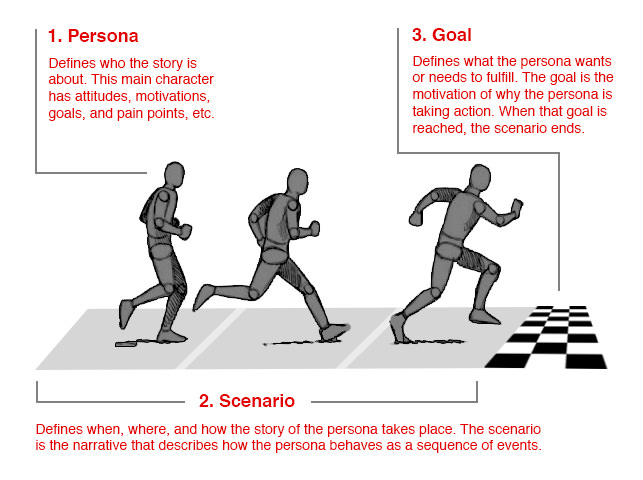
\includegraphics[scale=0.5]{goal-directed-perspective.jpg}
            \caption{Goal-directed persona perspective}
            \label{fig:goal-directed-persona-perspective}
        \end{figure}
    \subsubsection{The role-based persona}
    The role-based perspective is also a goal-directed perspective, but they are mainly focused on the role of the user inside the organization. A role-based persona should give an answer to the following questions.
    \begin{itemize}
        \setlength\itemsep{-2pt} 
        \item{Where will users use our product?}
        \item{What is the purpose of the product?}
        \item{What business objectives are required and what can be achieved with them?}
        \item{Which people will be impacted by its role?}
        \item{What kind of functions are being served?}
    \end{itemize}
    
    \subsubsection{The engaging persona}
    
    The engaging personas are distinguished by their very realistic persona descriptions. The other persona types tend to be too stereotypical, the designers are not able to envision their lives. Engaging personas are therefore specifically designed so that the designers who use them can become more engaged with them.
    
    \section{User stories}
    A key component of agile development is putting people first. A user story is a description of an end goal from a user's perspective. It's purpose is to articulate how a piece of work will return great value back to the customer. Note that "customers" don't have to be the end users. This can also be a colleague who depends on your team.
    
    Important to understand is that user stories are not a way to write requirements. The user stories help us start the right conversation about the users' needs, but don't go into detail. Eventually requirements are added once they are agreed upon by the team.
    
    \subsection{User story templates}
        User stories are often created based on a template. The most common template is the Connextra template or the three-part user story template. It highlights the who, the what and the why from the user's perspective. This template will also be used further down the paper.
        
    \begin{minted}{javascript}
        As a <role> I can <capability>, so that <receive benefit>.
    \end{minted}
    
    \begin{itemize}
        \item{\mintinline{javascript}{As a <role>} is often misinterpreted. A role is not a profession or job title, but a user persona. It is therefore important that the team has a shared understanding of this user persona. They should understand what he is working on, what he thinks and what he feels.}
        \item{\mintinline{javascript}{I can <capability>} describes the intent, not the features they use. What are the users trying to achieve? If you're describing any part of the \gls{ui} and not what the user's goal is, you are incorrect.}
        \item{\mintinline{javascript}{so that <receive benefit>} describes the user's end goal. This clause is seen as optional but often very helpful. In complex environment it will improve the general description of the user story.}
    \end{itemize}  
         
    The creator of the Connextra template, \href{https://en.wikipedia.org/wiki/Mike_Cohn/}{Mike Cohn}, recently wrote an article about why you should use the three-part template. Here is the link to the article:  \url{https://www.mountaingoatsoftware.com/blog/why-the-three-part-user-story-template-works-so-well}.
    
   \section{User flow}
    A user flow is a series of actions a prototypical user takes to accomplish a certain goal. 
    Projects often have many stakeholders, requirements and limitations causing the user not being the central role in the design. By making user stories, we don't only ensure that the user remains the point of focus but it is a great tool for developers to show how the product or service should work.
    
    \section{Prototyping}\label{sec:prototyping}
    A prototype is a rudimentary working sample of a product or service built to test if a certain concept or process works. It is a low cost way to reduce the risk that the idea may not perform as intended, however generally it cannot eliminate all risk. Prototyping helps you assure that only the best version of something goes forward.
    
    Prototyping has several important benefits: 
    \begin{itemize}
        \item {You receive valuable feedback from the users early in the process.}
        \item { Compared to development, prototyping is a very efficient and effective process, especially when several rounds are required to fine-tune the outcome. }
        \item {Prototypes are a great way to check if the customer's requirements correspond to the design. }
        \item {Completed prototypes allow the software engineers insight into the accuracy of initial project estimates and whether the proposed deadlines and milestones can be met.}
        
    \end{itemize}
    
    \section{Usability testing} 
    Usability testing involves watching representative users working with your product or service so that you can make improvements based on their actions. Usability testing gives you invaluable feedback on how users behave with your product or service. Knowing how your users behave helps you create a much suitable product or service. 
    Rather than guessing about what your users might like or need, you can see their usage first handed. 
    
    \subsection{Moderated usability testing}  
    Moderated usability testing is when the user completes a set of tasks, while being observed by a moderator (researcher).
    Moderated usability has many benefits: 
    \begin{itemize}
        \setlength\itemsep{-2pt} 
        \item { You receive immediate feedback, so that important details are not lost.}
        \item { You can answer any immediate question posed by the user.}
        \item { You have the ability to guide users through tasks.}
        \item { Early prototyping may contain unfinished features which can cause confusion. By being physically present you can clarify on the spot.}
        \item { You have an overview on all tasks the user performs, both active and passive.}
    \end{itemize} 
    
    However, moderated usability testing has a major drawback. It is greatly affected by the Hawthorne effect.

    \subsubsection{The Hawthorne effect}
    The Hawthorne effect occurs when people behave differently because they know that they are being observed. The term was first introduced by H. A. Landsberger who was conducting research at the Hawthorne Works factory. The factory wanted to investigate whether the employees would become more productive with higher light intensities. 
    
    At first the productivity seemed to have increased considerably, but it completely plunged after the experiment ended. The production gain was due to the motivational effect. The workers performed better because of the interest that was being shown in them.
    
    \section{Design handoffs}
    A Design handoff is the moment the designers have finished their work and deliver the results to the developers. A design handoff is preferably not the design itself but dedicated spec files. Spec files can often be generated by the design tool or third party plugins.
    
    
    The goal of handoffs is to eliminate guesswork and make the developers experience as easy as possible. 
    Design handoffs should not be a way to prevent communication between designers and developers. 
    